\section{Messprotokolle}

\begin{figure}[!ht]
 \centering
 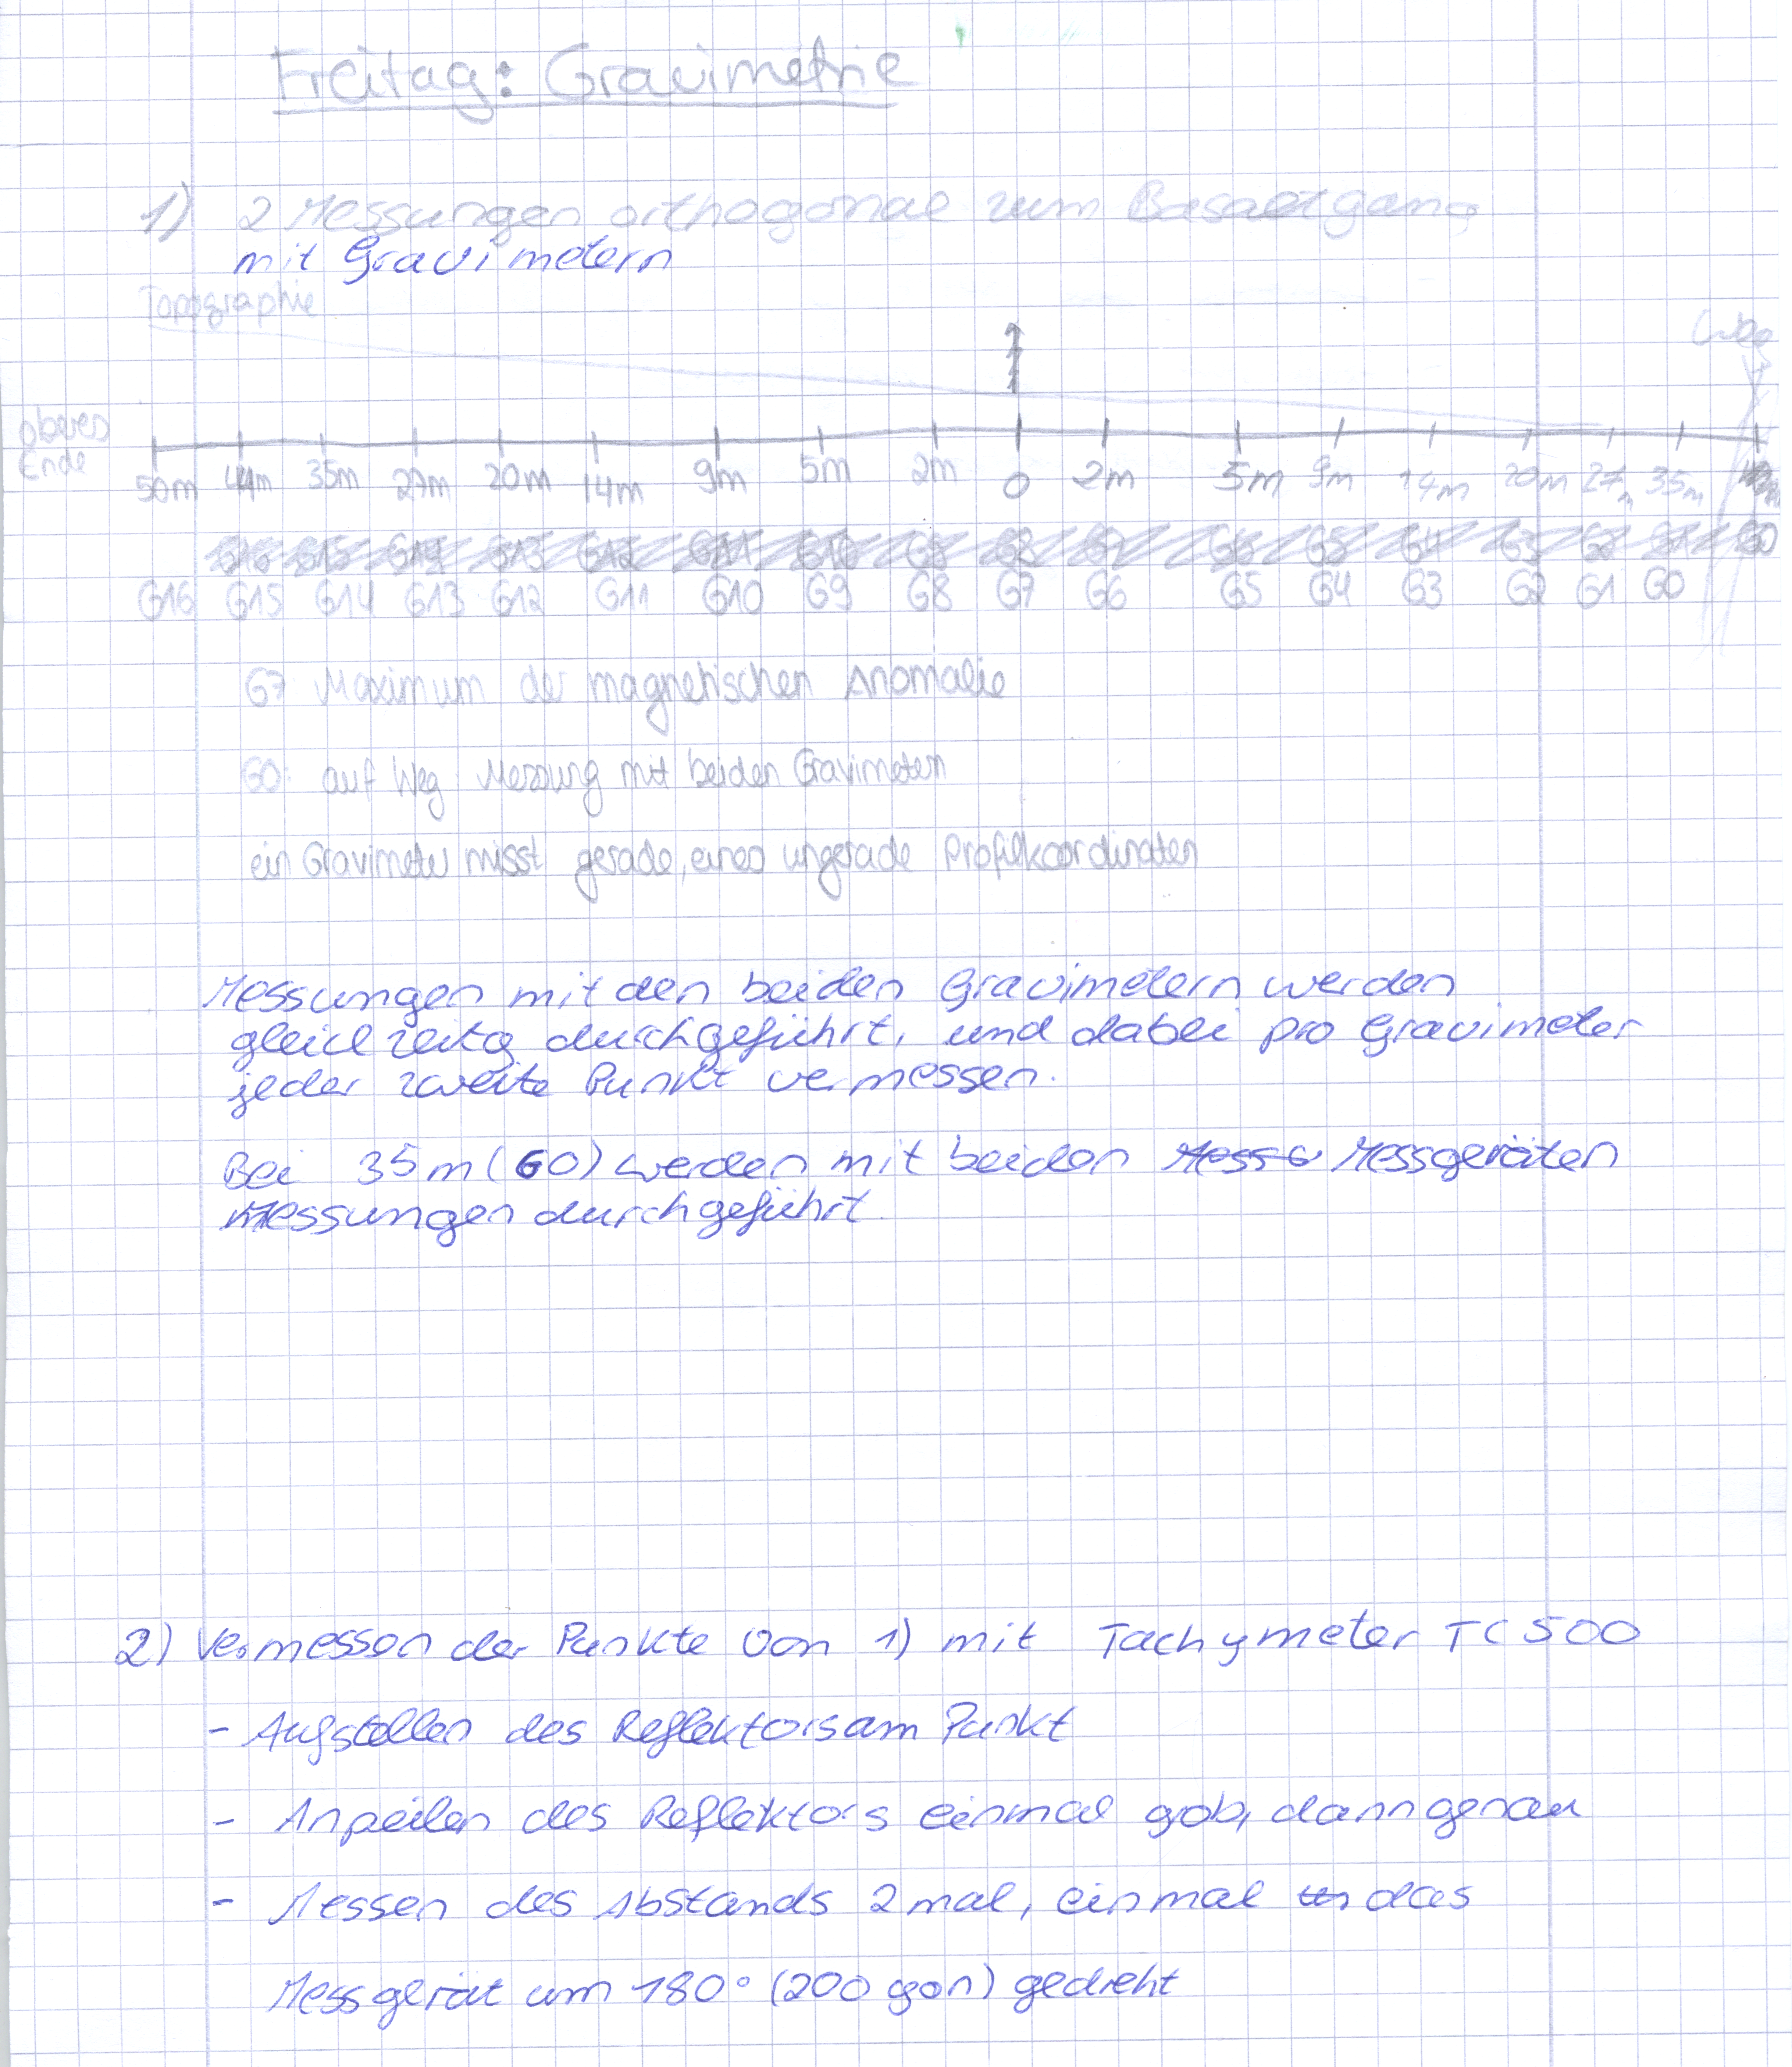
\includegraphics[width=0.9\textwidth]{fig/Messprotokolle/Versuchsbeschreibung1}
 \caption{Versuchsmitschrieb 1}
 \label{fig:mitschrieb1}
\end{figure}

\begin{figure}[!ht]
 \centering
 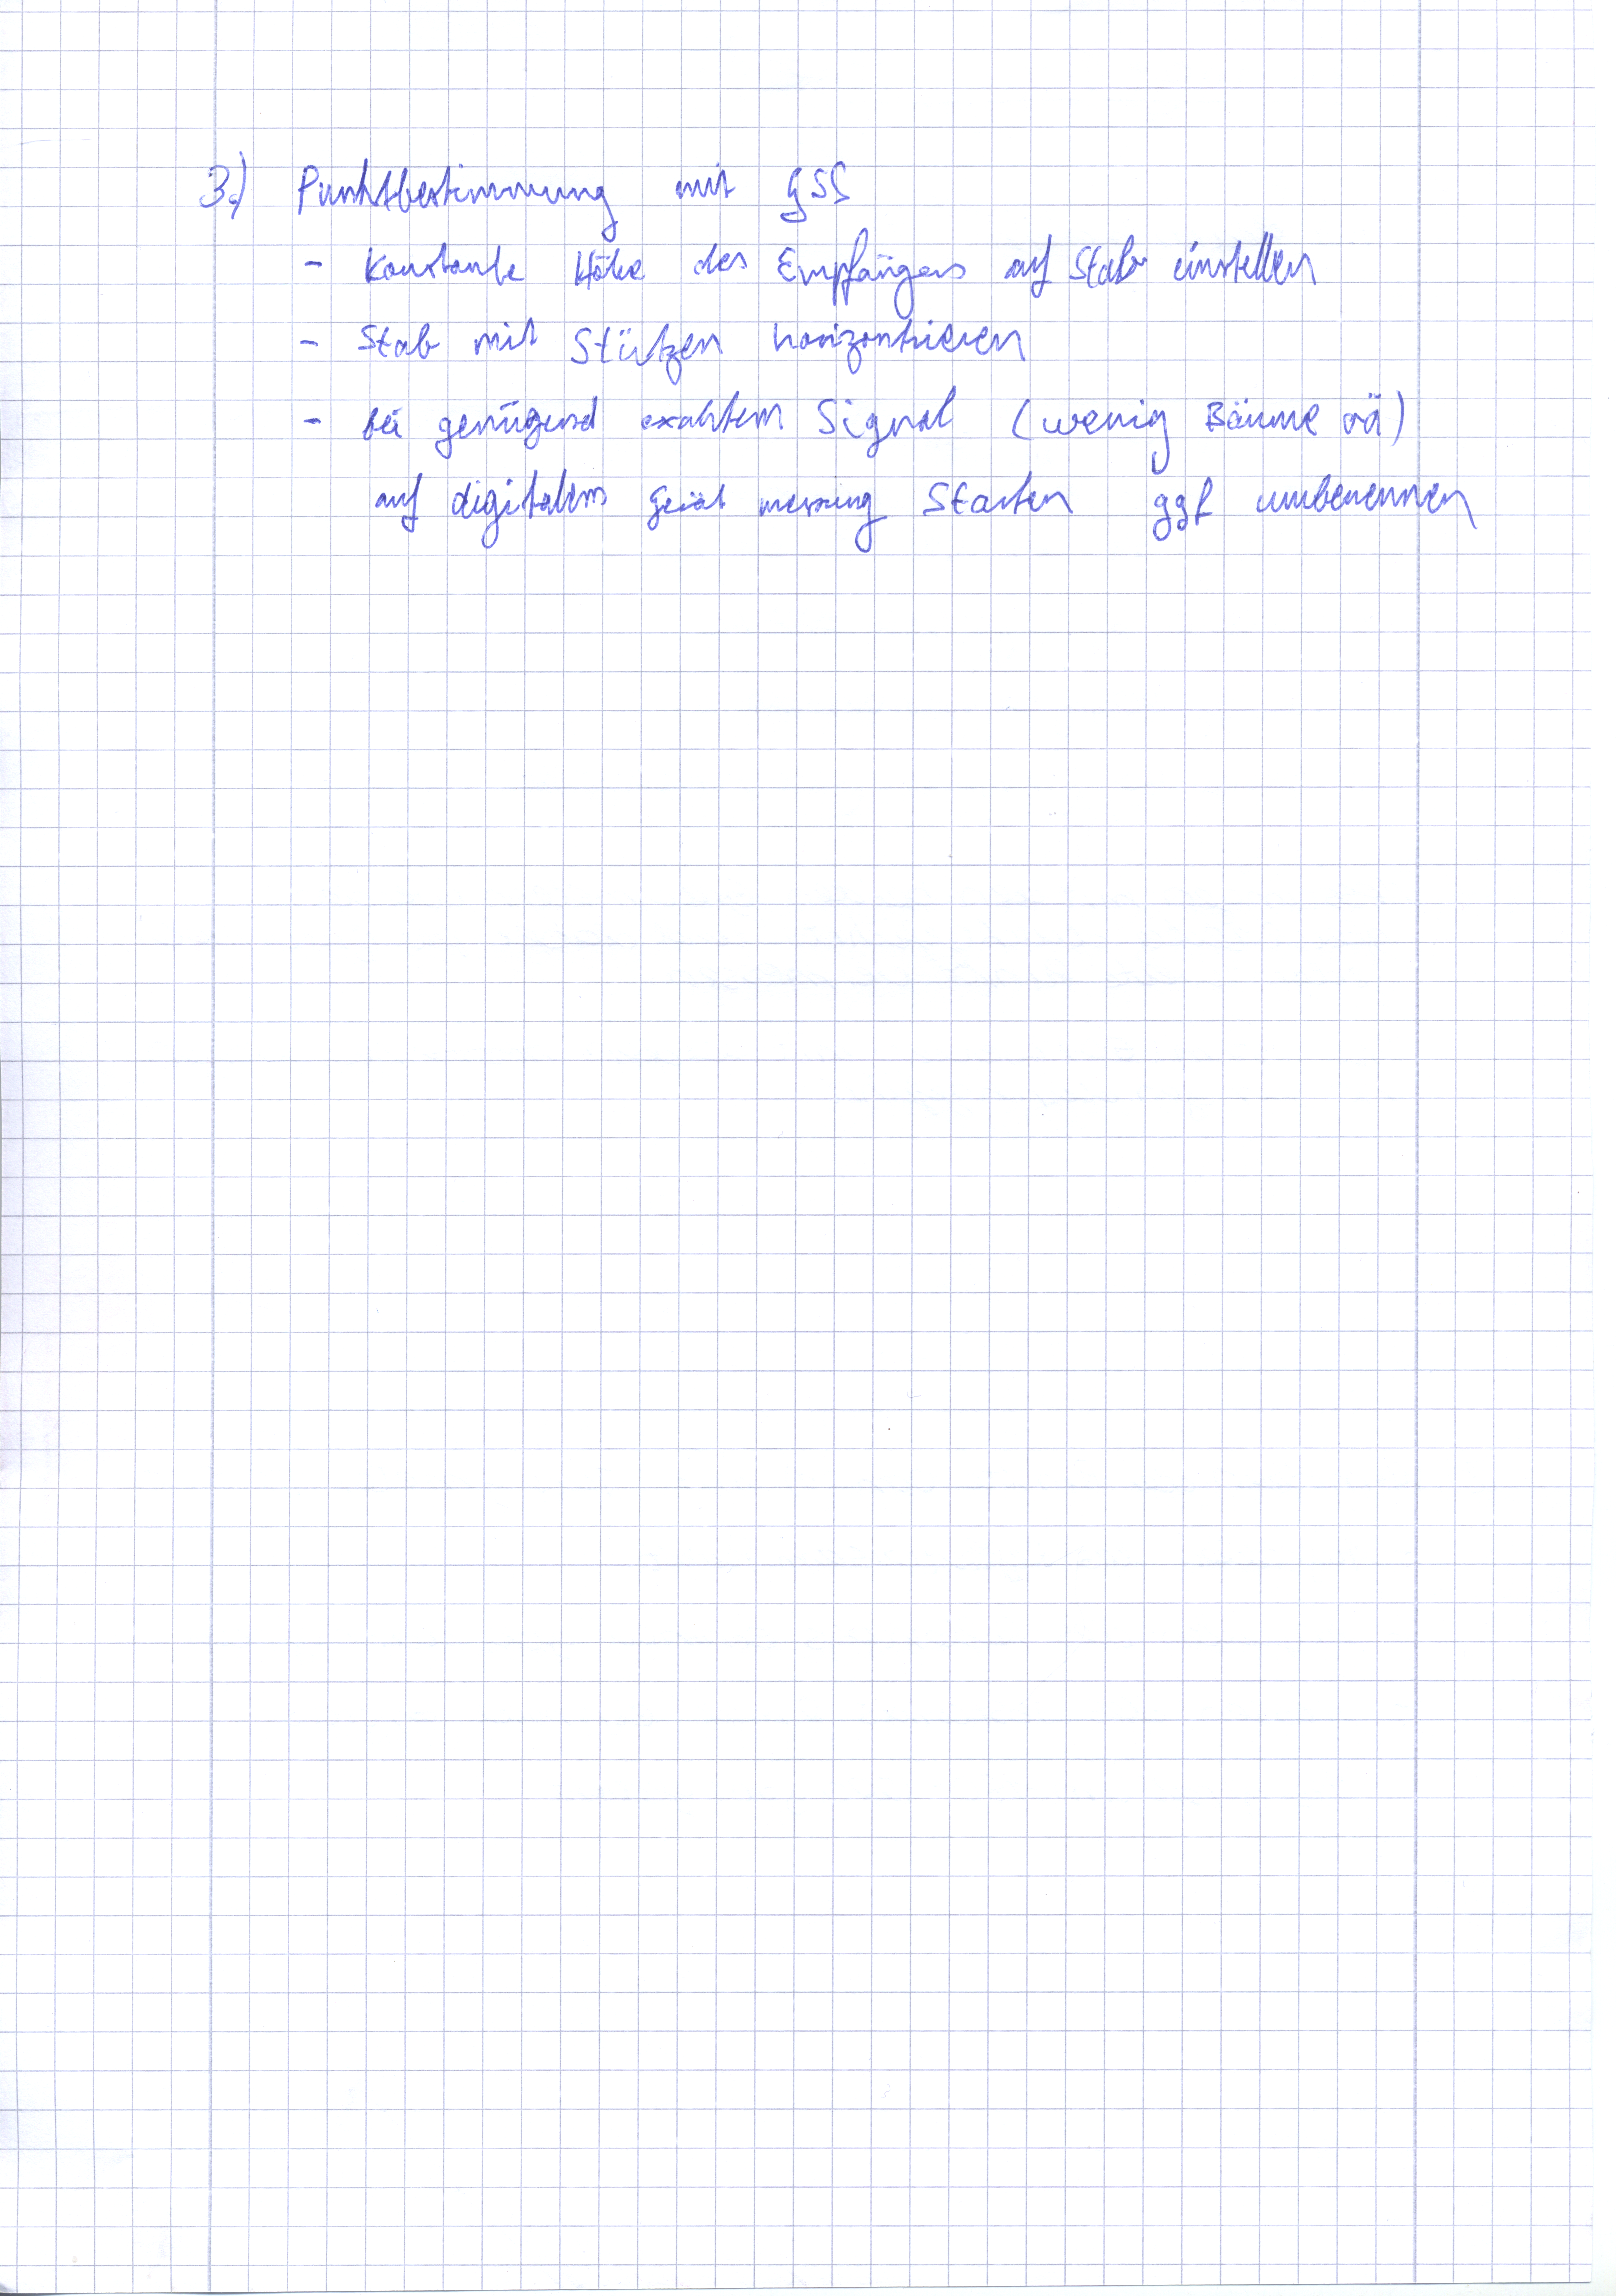
\includegraphics[width=\textwidth]{fig/Messprotokolle/Versuchsbeschreibung2}
 \caption{Versuchsmitschrieb 2}
 \label{fig:mitschrieb2}
\end{figure}

\begin{figure}[!ht]
 \centering
 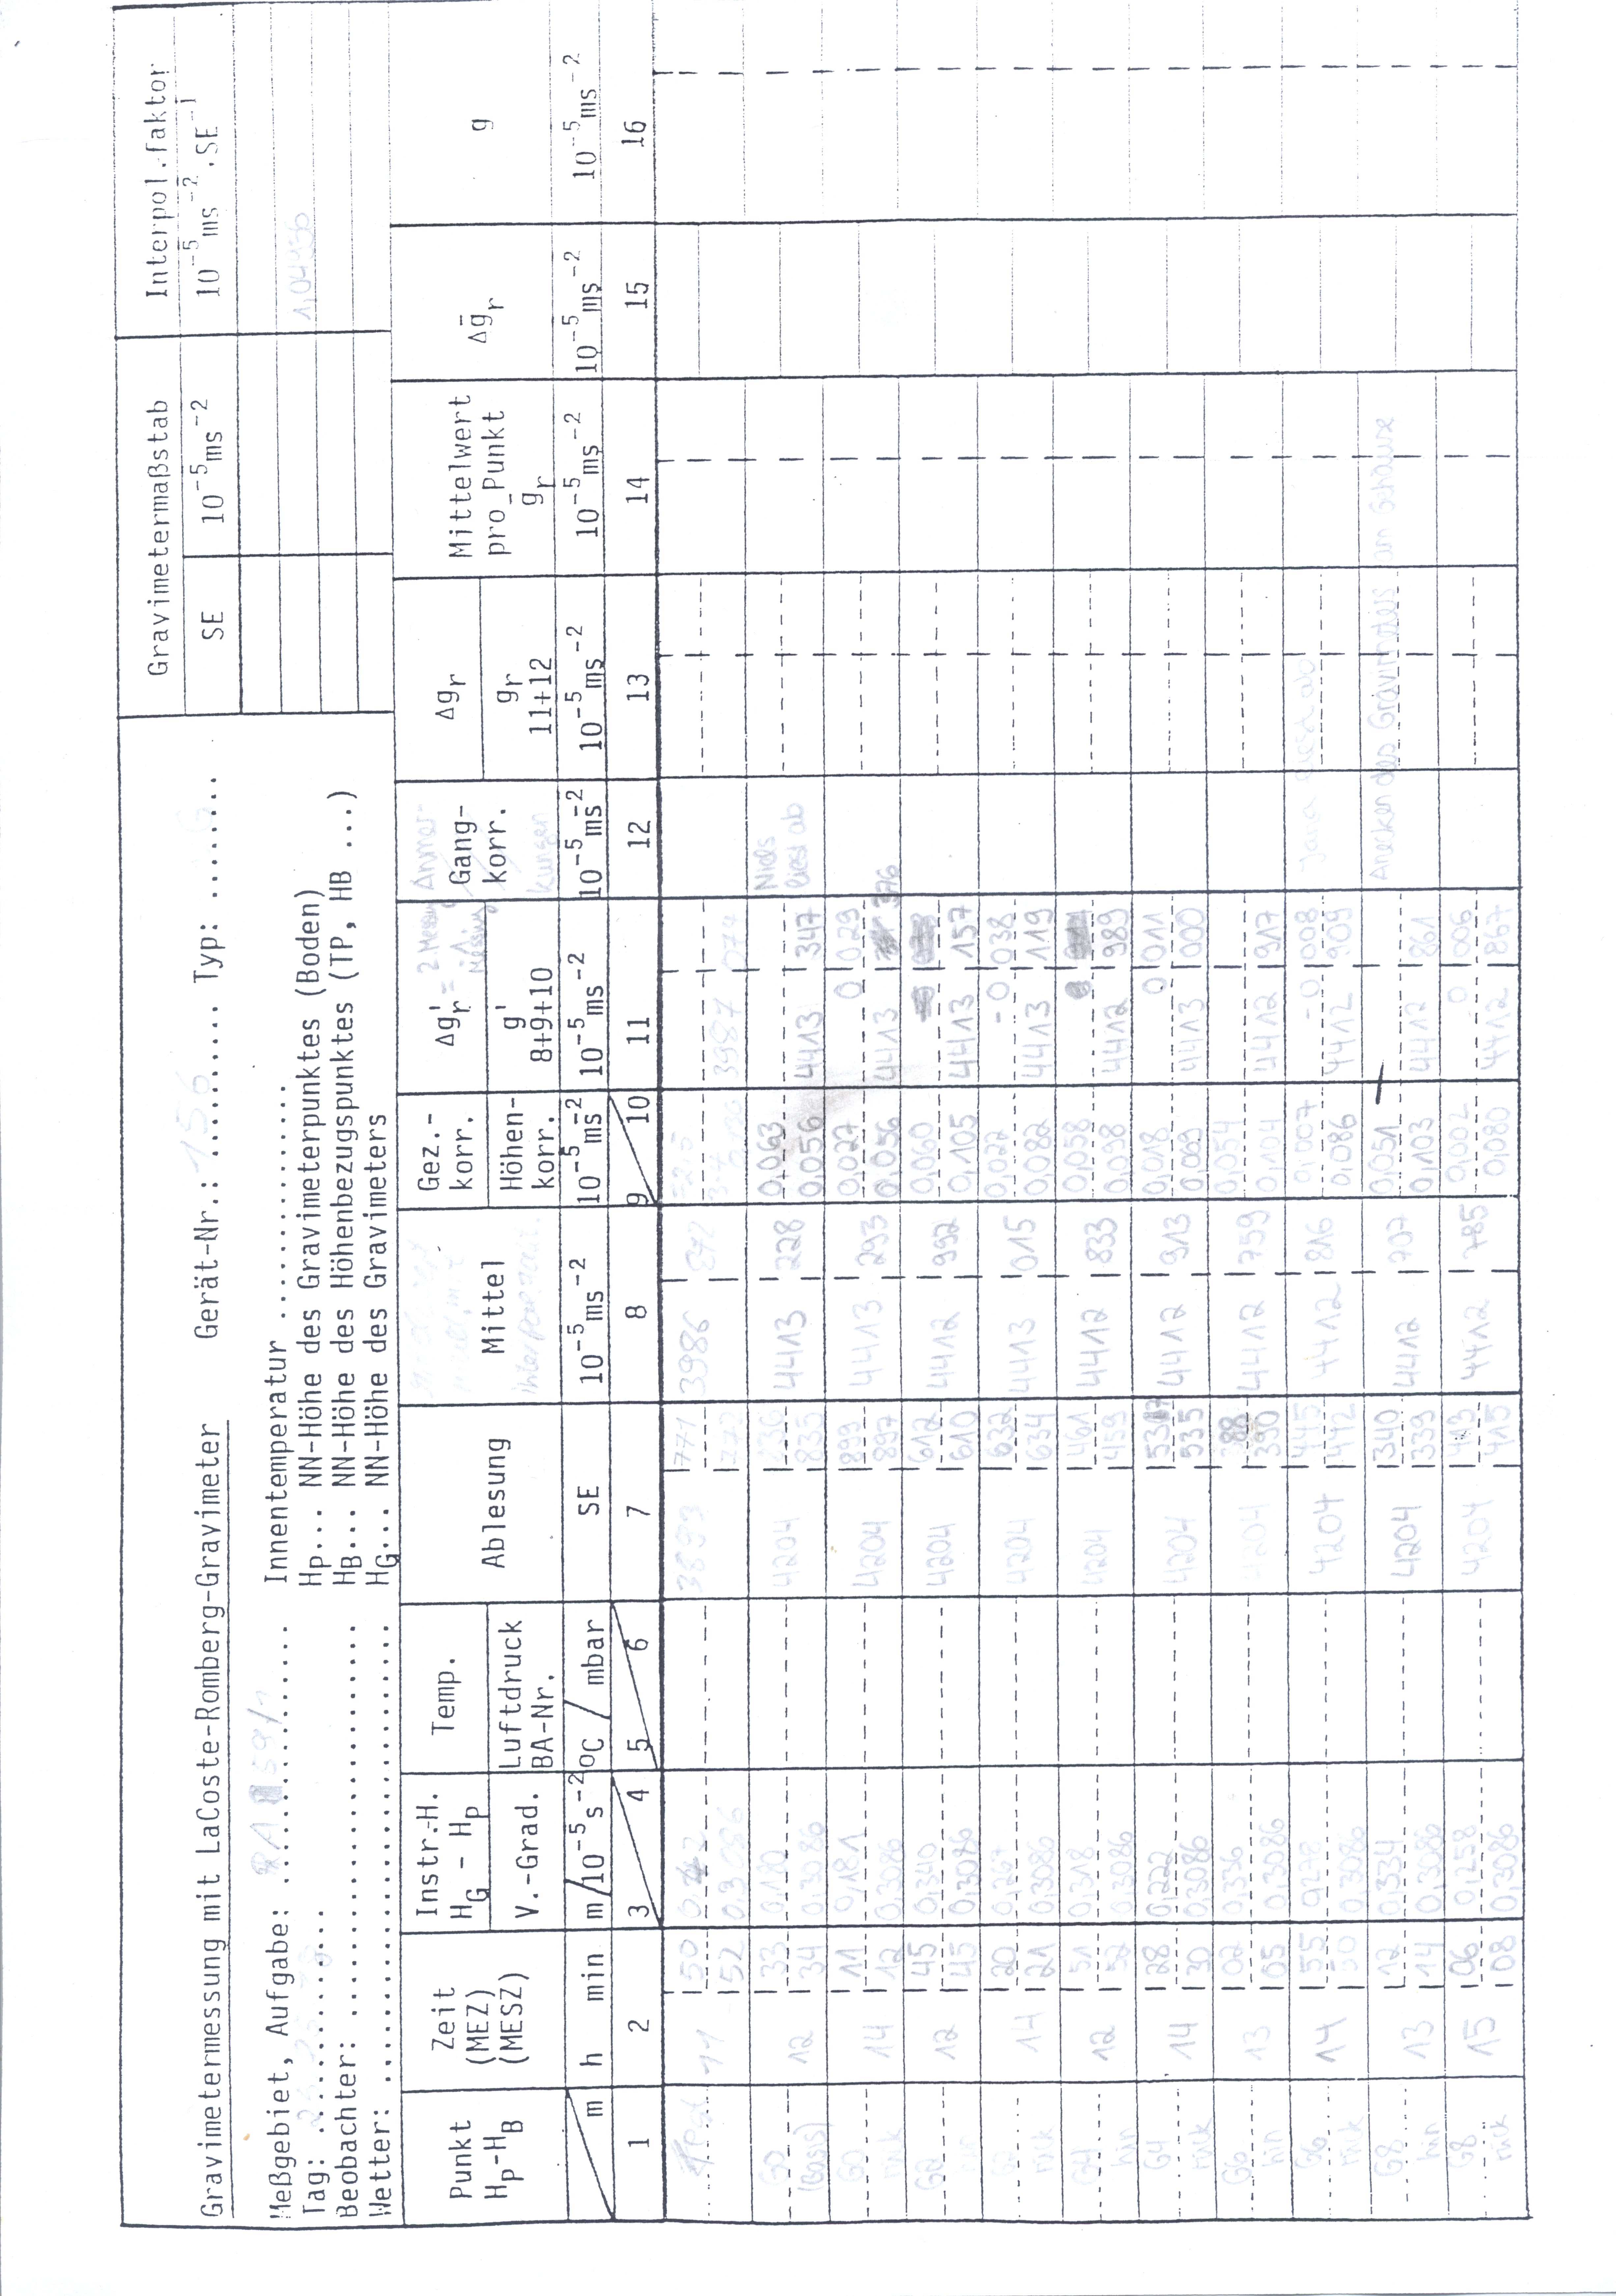
\includegraphics[width=\textwidth]{fig/Messprotokolle/Messprotokoll1-156g}
 \caption{1. Messprotokoll der Messungen mit Gerät Nr. 156 Typ G}
 \label{fig:MP1_156}
\end{figure}

\begin{figure}[!ht]
 \centering
 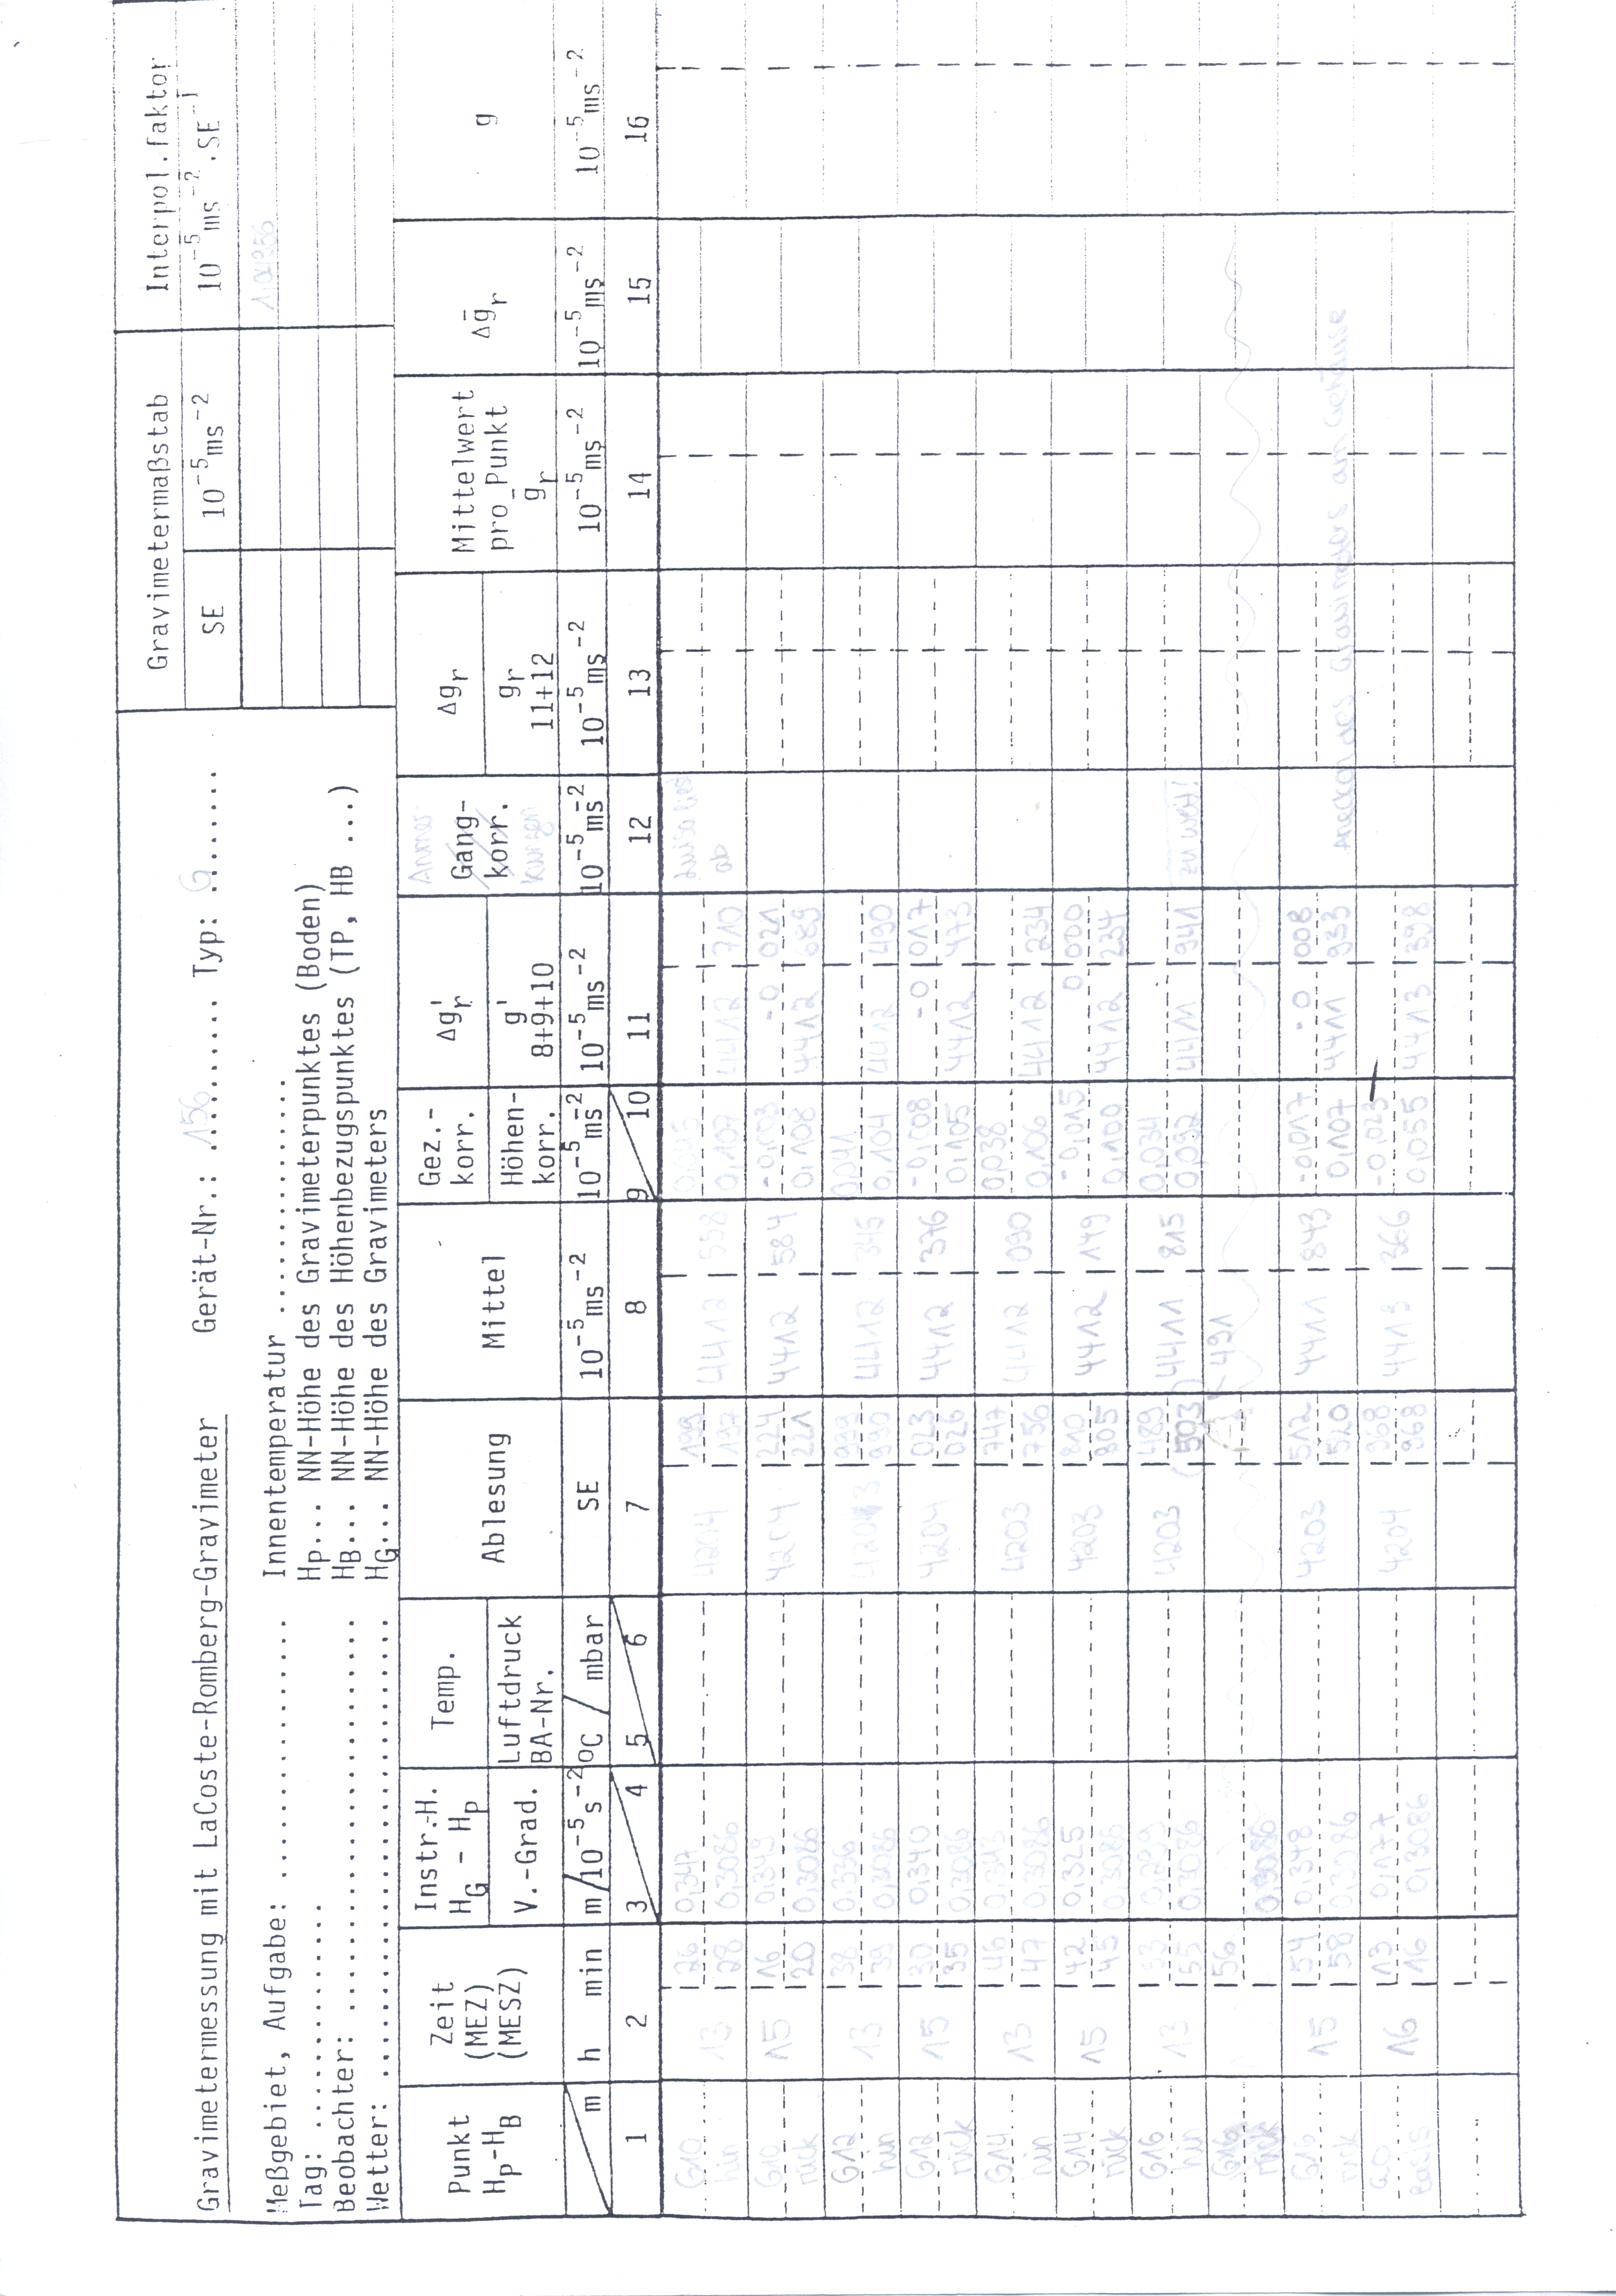
\includegraphics[width=\textwidth]{fig/Messprotokolle/Messprotokoll2-156g}
 \caption{2. Messprotokoll der Messungen mit Gerät Nr. 156 Typ G}
 \label{fig:MP2_156}
\end{figure}

\begin{figure}[!ht]
 \centering
 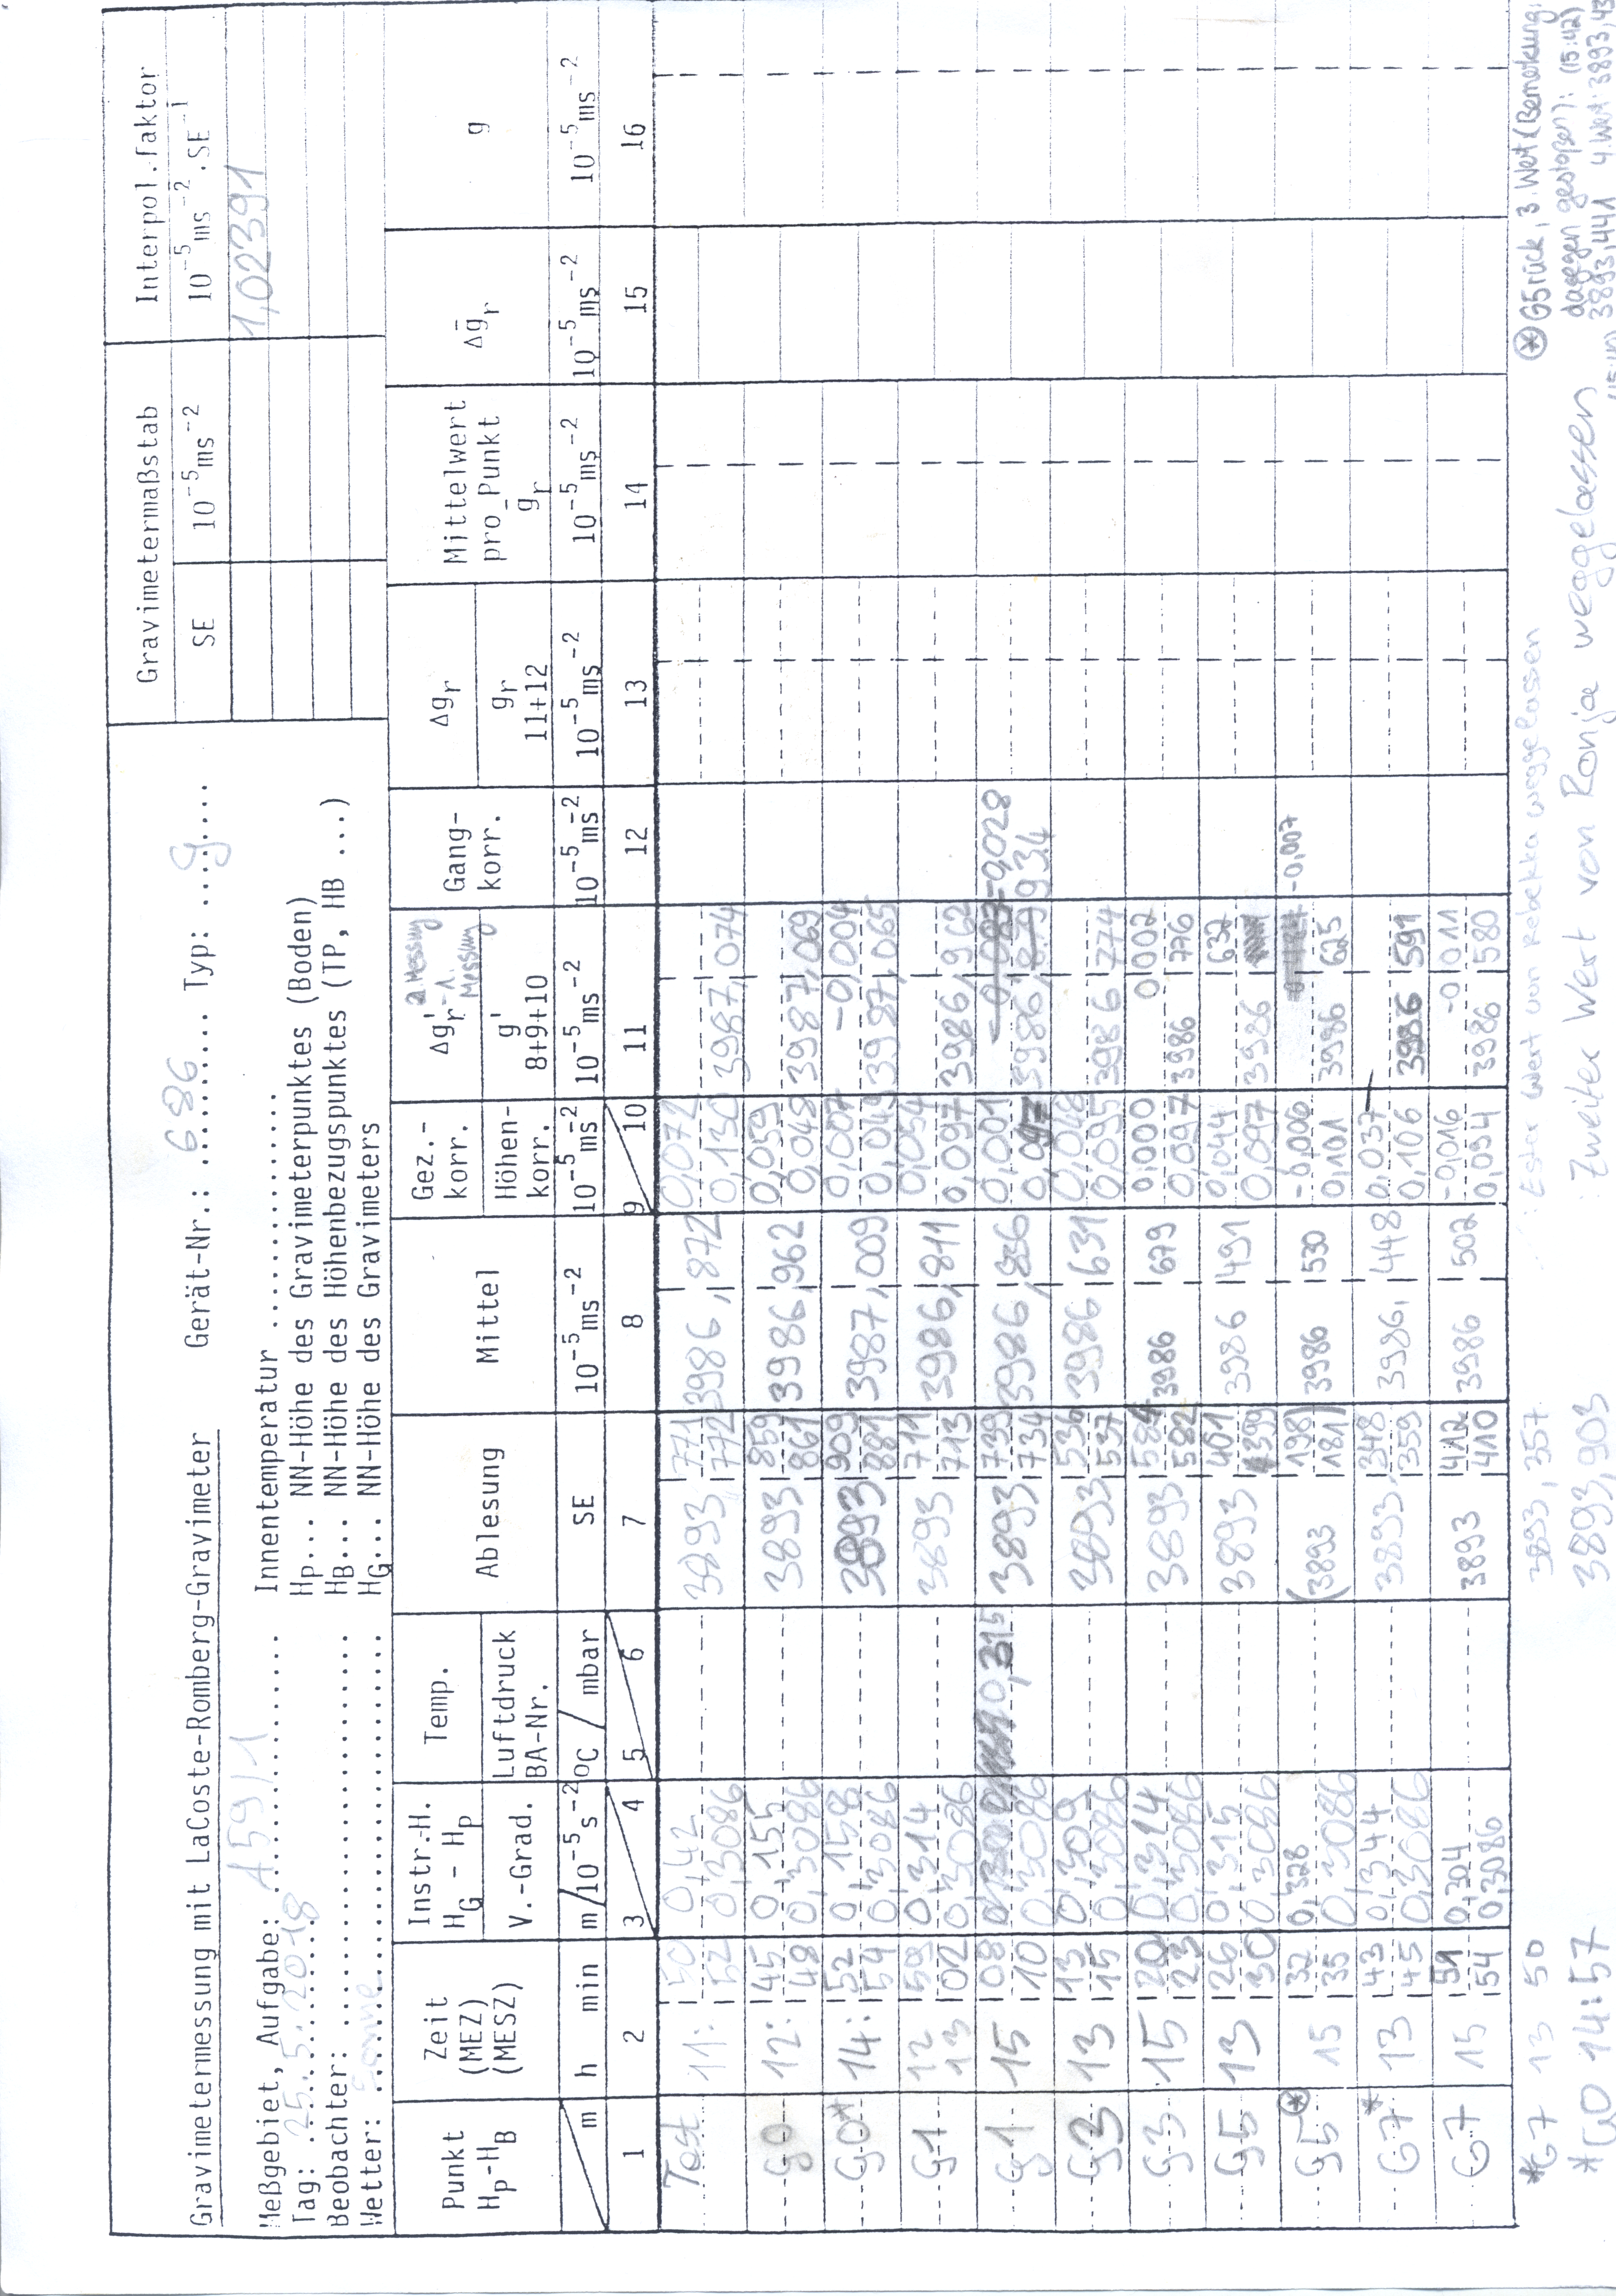
\includegraphics[width=\textwidth]{fig/Messprotokolle/Messprotokoll1-686g}
 \caption{1. Messprotokoll der Messungen mit Gerät Nr. 686 Typ G}
 \label{fig:MP1_686}
\end{figure}

\begin{figure}[!ht]
 \centering
 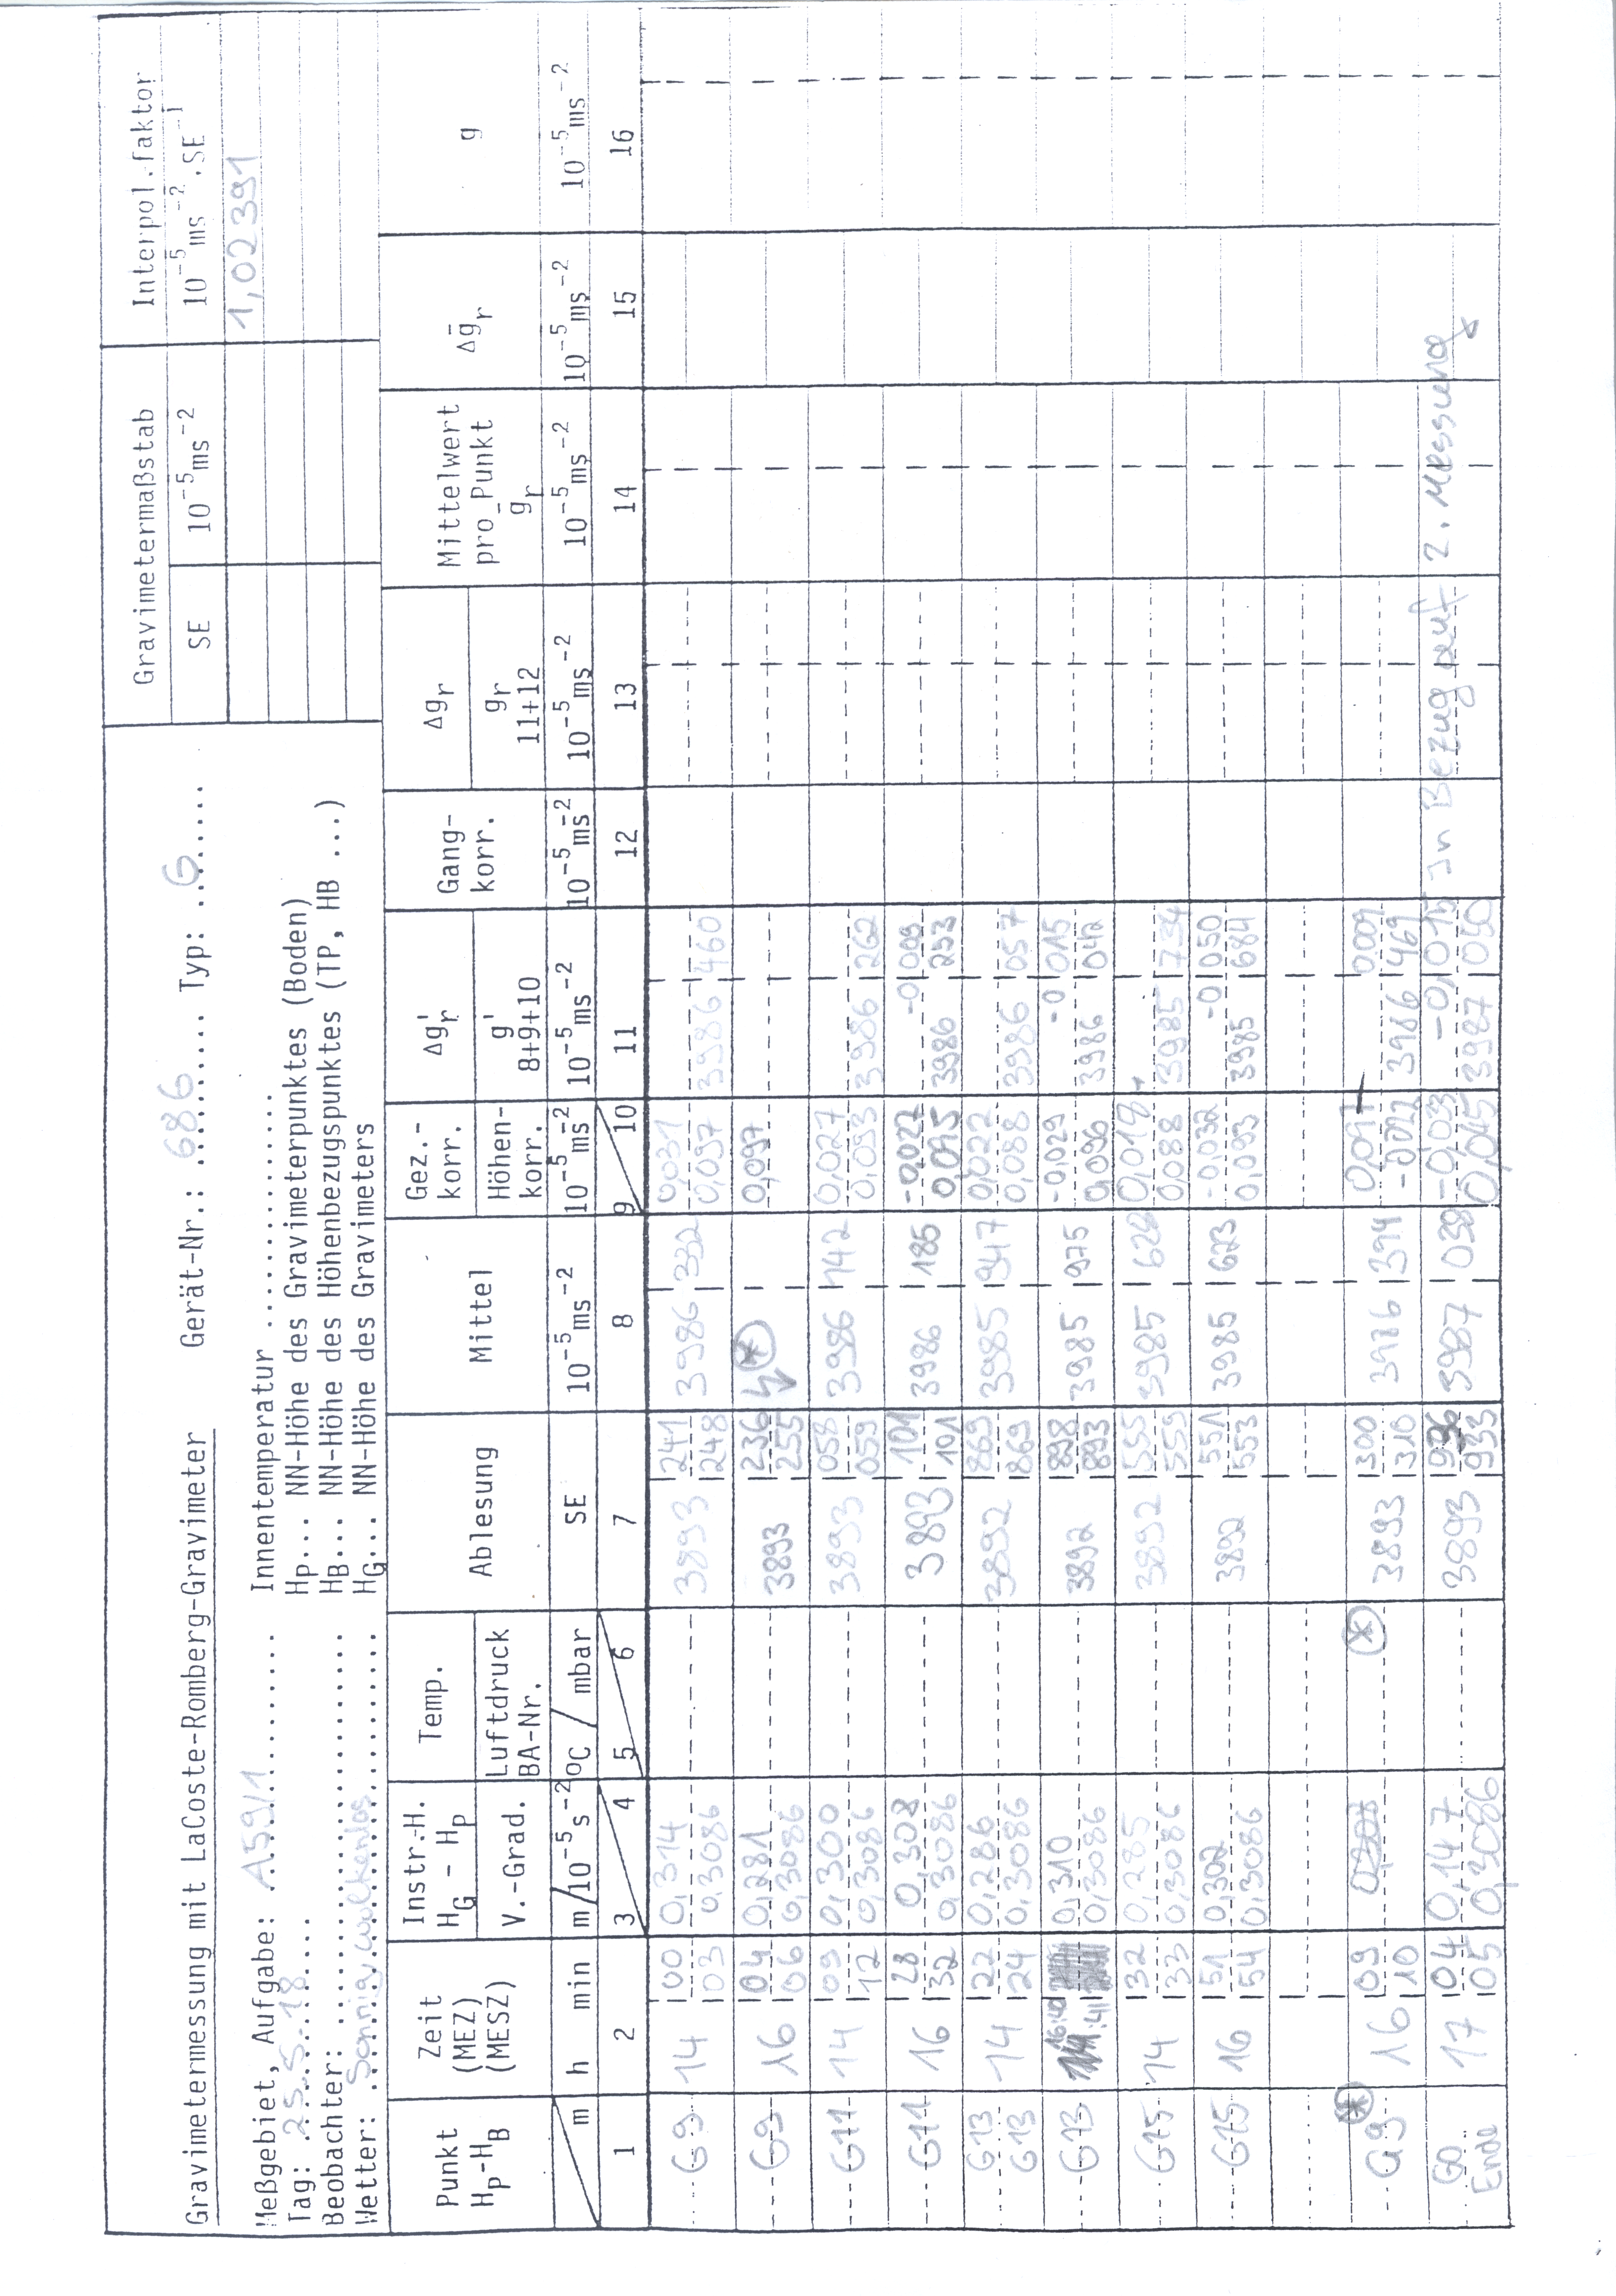
\includegraphics[width=\textwidth]{fig/Messprotokolle/Messprotokoll2-686g}
 \caption{2. Messprotokoll der Messungen mit Gerät Nr. 686 Typ G}
 \label{fig:MP2_686}
\end{figure}

\begin{figure}[!ht]
 \centering
 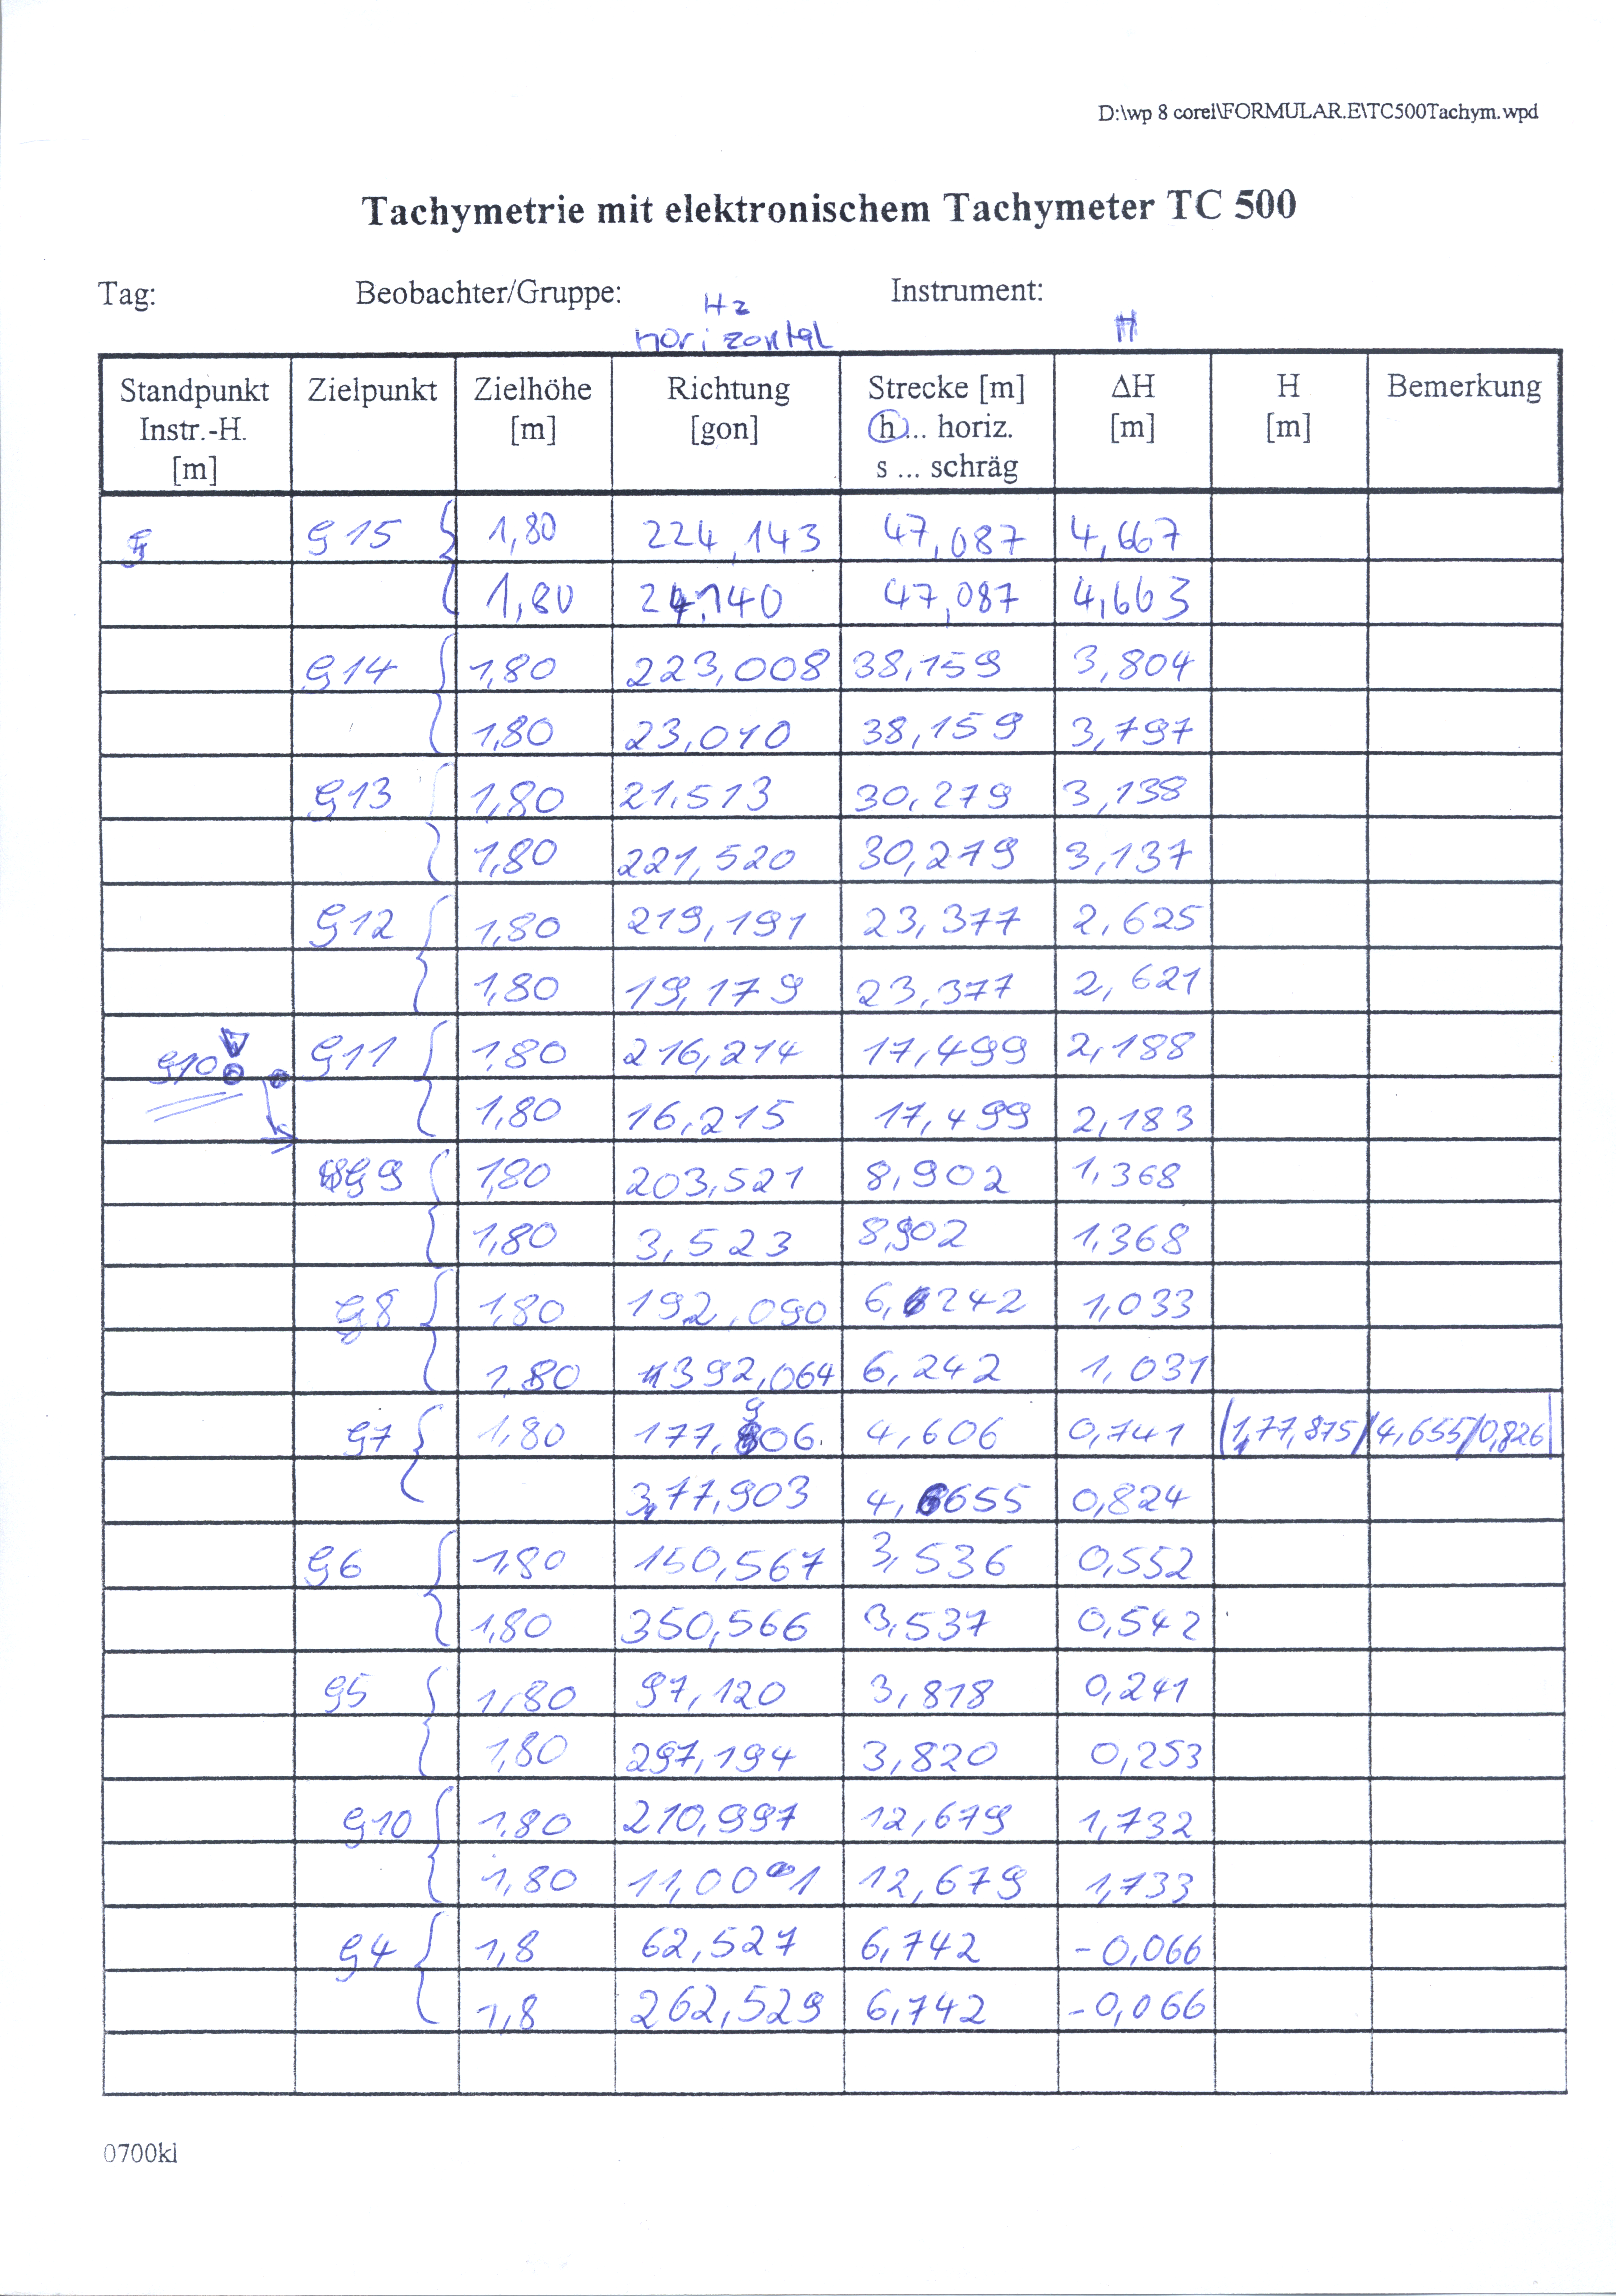
\includegraphics[width=\textwidth]{fig/Messprotokolle/Tachymetrie1}
 \caption{1. Messprotokoll zur Tachymetrie}
 \label{fig:MPTachymetrie1}
\end{figure}

\begin{figure}[!ht]
 \centering
 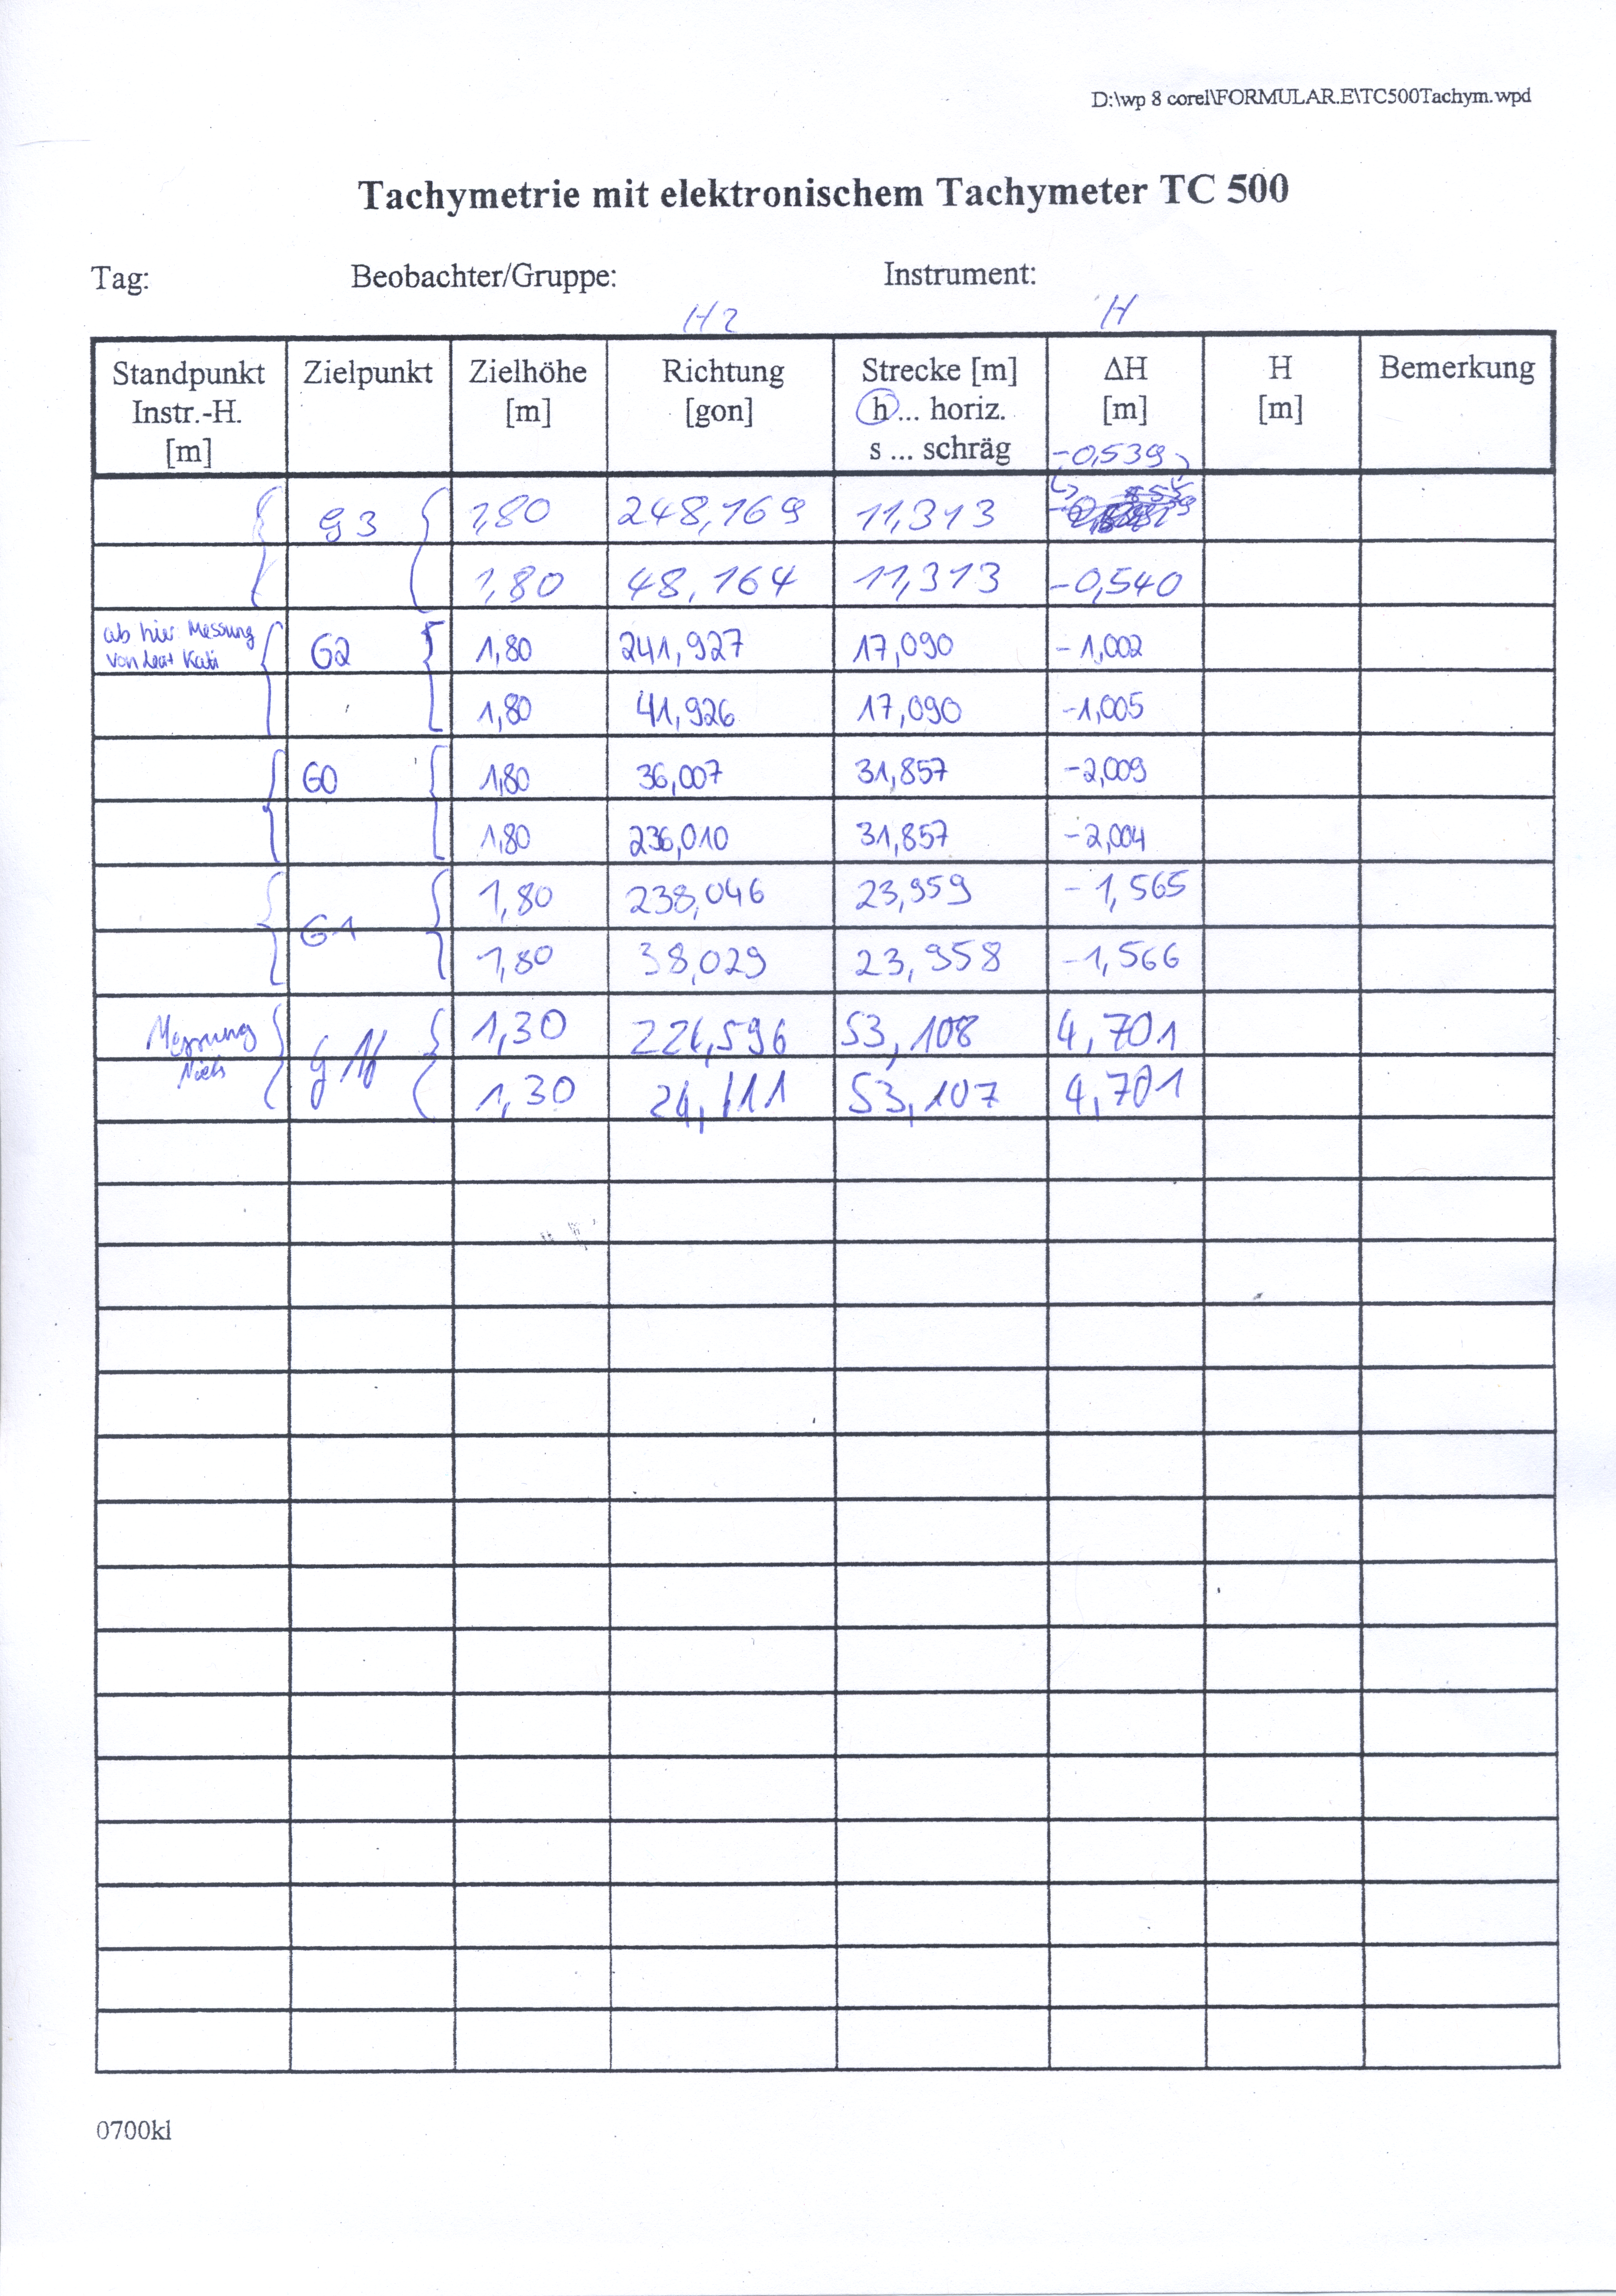
\includegraphics[width=\textwidth]{fig/Messprotokolle/Tachymetrie2}
 \caption{1. Messprotokoll zur Tachymetrie}
 \label{fig:MPTachymetrie2}
\end{figure}

\begin{figure}[!ht]
 \centering
 \includegraphics[width=\textwidth]{fig/Messprotokolle/schlumberger_sondierung.bmp}
 \caption{thw}
 \label{fig:}
\end{figure}

% \begin{figure}[!ht]
%  \centering
%  \includegraphics[width=\textwidth]{fig/Messprotokolle/}
%  \caption{}
%  \label{fig:}
% \end{figure}